    \begin{wrapfigure}{R}{0.4\textwidth}
    	\begin{center}    		
    		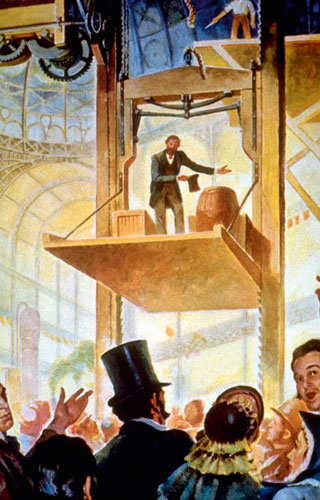
\includegraphics[scale=0.5]{img/Otis_Safety_Elevator}
    	\end{center}
    	\caption*{Otis Spectacle}
    	\label{Otis_spectacle}
    \end{wrapfigure}  
	The invention of the elevator was a precondition for the invention of 
	skyscrapers, given that most people would not (or could not) climb more 
	than a few flights of stairs at a time. For most people, when they 
	finished climbing 7 floors
	then they would be out of breath. (PS: Since secondary school, I've 
	invariably been living 
	in the top floors of dormitory buildings, which had 6 or 7 floors but 
	without any elevators 😂. Unbelievable!!) So, the occurrence of  
	elevators, though not technically, fairly boost the development of  
	skyscrapers. People hate climbing stairs! In modern world, it's  
	unimaginable to consider a building without any elevators, even a 
	building of seven stories high (e.g. a residential building, 
	a library, etc.). 
	
	In the 1800s, elevators that operated on a cable system were deemed 
	unreliable and dangerous, because, if the ropes broke, the elevator 
	plummeted to the bottom. Freight could be damaged, but, more importantly, 
	passengers were often killed by the fall. Scary, isn't it? Then some 
	brilliant mechanic named \textbf{Elisha Otis} invented a safety elevator 
	that 
	prevent the destruction.
	
	While working in a factory in 1852, Elisha Otis and his sons came up with 
	an elevator design that employed a safety device. A wooden frame at the 
	top of the platform would snap out against the sides of the elevator shaft 
	if the ropes broke, essentially functioning as a brake. Otis called it the 
	``\emph{safety hoist}" and dramatically demonstrated this design at the 
	1854 New York World's Fair (see picture
	\hyperref[Otis_spectacle]{Otis Spectacle}).
	He rode the platform high 
	into the air and then had the 
	rope cut, but, thanks to the brake, it only fell a few inches before 
	stopping. Otis founded an elevator company, Otis Brothers, which installed 
	the first public elevator in a five-story New York department store in 
	1874. Electric elevators came about in the 1880s. 
	
	And now the Otis Elevator Company is the world's largest manufacturer of 
	vertical transportation systems, principally focusing on elevators, moving 
	walkways, and escalators.\\[3pt]
	
	Nowadays, there are four main types of elevators: hydraulic, traction, 
	machine-room-less, and vacuum. \textbf{
	In this article, we merely discuss
	traction elevators}. View the differences among these types 
	of elevators \href{
	https://www.vacuumelevators.com/a-guide-for-choosing-the-type-of-elevator-you-need/}
	{here}.\\[3pt]
	
	For more information about the history of elevators see 
	\url{http://otiselevator.umwblogs.org/adoption/}, 
	\url{https://www.cnn.com/style/article/short-history-of-the-elevator/index.html},
	 \&
 	\url{https://science.howstuffworks.com/innovation/inventions/who-invented-the-elevator1.htm}.
 	
 	There are also a couple of YouTube videos that I downloaded \& uploaded to 
 	my website, view history part
 	\href{https://markjohntaylor.com/blog/wordpress/index.php/2020/06/15/the-elevator#history}{here}.
	 	
	\clearpage 